% flat-plate.tex
\newpage
\section{Flat plate}
\label{chapter-flat-plate}
%
The first validation test case is that of a two-dimensional Mach 3.7
flow over a flat plate. In this exercise, Eilmer3 simulation results are compared to
the experimental results of Coles \cite{Coles1953} \footnote{These experimental
results are presented as case number 53010801 in Fernholz \& Finley 
\cite{Fernholz1977}} and van Driest's \cite{vanDriest1956} theoretical correlation 
for skin friction on a flat plate. This exercise also explores the $k$-$\omega$ 
model's sensitivity to the given freestream turbulence properties.

%------------------------------------------------------------------
\subsection{Details of flow problem}
\label{flat-plate-flow-problem}
%
The experimental setup used by Coles was basically a flat plate model
installed 13\,mm below the tunnel centreline in the test section of
the 20-inch supersonic wind tunnel at the Jet Propulsion Laboratory in the California Institute of Technology.
The overall length and width of the plate were 0.84\,m and 0.46\,m
respectively, with the lower surface of the plate being the test surface. 
The boundary layer was tripped by a wire fence trip at the model leading 
edge and was assumed to turbulent right from the leading edge.
This experiment has been classified by Fernholz \& Finley \cite{Fernholz1977} as a
zero-pressure-gradient, adiabatic-wall,flat-plate test case.
The nominal inflow conditions are given in Table~\ref{inflow-conditions-table1}.
%
\begin{table}[h]
  \caption{Nominal inflow conditions for Coles' flat plate test case}
  \label{inflow-conditions-table1}
  \begin{center}
    \begin{tabular}{cccl}
      \hline\hline
      Parameter & Value   & Units \\
      \hline
      $M_\infty$  & 3.7     &     \\
      $p_\infty$  & 1.358e3 & Pa  \\
      $T_\infty$  & 83.34   & K   \\
      $u_\infty$  & 677.4   & m/s \\
      \hline \hline
    \end{tabular}
  \end{center}
\end{table}
%
Boundary layer profiles of pitot pressure were
experimentally measured at 0.546\,m downstream of the leading edge.
Profiles of temperature, velocity and density were then derived using
the Crocco/Van-Driest temperature-velocity relation with the
assumption of constant static pressure throughout the boundary layer.
Although the uncertainties of the experimental and derived data were not
specified by Coles, theoretical correlations can be used to support this 
validation exercise. A compressible turbulent boundary layer has been 
shown to follow the semi-empirical logarithmic law of the wall
velocity profile that is similar to its incompressible counterpart \cite{Smits2006}.
In addition, the turbulent skin friction theory of van Driest \cite{vanDriest1956} is used for comparison
with the computed skin friction coefficient values along the flat plate.
An estimation of the accuracy of this theory ranges from $\pm$3\% \cite{Squire2000}
to $\pm$10\% \cite{Hopkins1971}.
%------------------------------------------------------------------
\subsection{Details of computational approach}
\label{flat-plate-computational-approach}
%
The computational mesh used is shown in Figure~\ref{computational-mesh},
with the NORTH boundary being the adiabatic wall, the EAST boundary being
the extrapolated outlet, and the SOUTH and WEST boundaries being the
supersonic inflow. The inflow parameters were specified as per
Table~\ref{inflow-conditions-table1}. Air with an ideal gas assumption, a
constant specific heats ratio of 1.4 and a gas constant of 287.1 J/kg.K was used
as the test gas for the simulations.
\begin{figure}[h]
 \begin{center}
  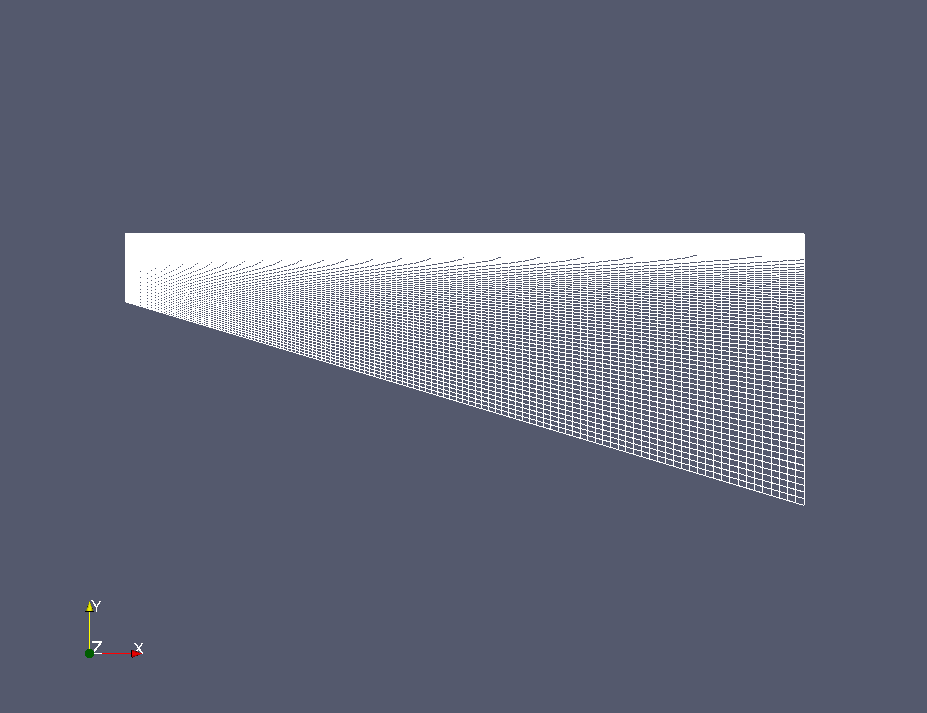
\includegraphics[width=10cm]{./chap2-flat-plate/figs/grid.png}
 \end{center}
 \caption{Computational mesh}
 \label{computational-mesh}
\end{figure}
Three sets of grids were used for this test case - a fine grid
(160$\times$140 cells), a medium grid (80$\times$70 cells), and a coarse (40$\times$35 cells).
The $y^+$ for the grids were lesser than 1.0, except in the first few wall
cells from the leading edge where the boundary layer was establishing.
It was also ensured that there were at least 15 cells within the
boundary layer for most parts of the computational domain.
%-----------------------------------------------------------------
\subsection{Grid convergence}
%\label{}
%
The grid spatial discretisation error can be estimated by using the
Richardson's Extrapolation procedure described in Roache \cite{Roache1998}. Being
the more sensitive parameter to grid refinement, the spatial discretisation
error of the skin friction coefficient is examined, as shown in
Figure~\ref{spatial-discretisation-error}. The value of the errors for all
three grids should follow the equality specified by Roy \& Blottner \cite{Roy2003} if
the mesh levels are sufficiently refined to be in the second-order asymptotic
range. In the turbulent region (beyond $x$ = 0.2 m), it can be seen that this equality
is satisfied, and that the spatial discretisation errors are below 0.5\% (check).
The high levels of spatial discretisation errors observed in the region between
$x$ = 0.0 m to $x$ = 0.15 m are brought about by the transitioning of the boundary layer
and the singularity at the leading edge of the plate. This effect has also been
observed by Roy \& Blottner \cite{Roy2003}. It can be assumed from this study that the solutions
are sufficiently grid-independent.
\begin{figure}[h]
 \begin{center} \vspace{1cm}
  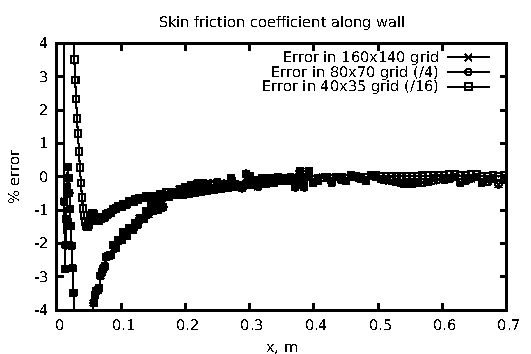
\includegraphics[width=10cm]{./chap2-flat-plate/figs/coles-x05-cf-error.pdf}
 \end{center}
 \caption{Grid convergence check}
 \label{spatial-discretisation-error}
\end{figure}
%\begin{figure}[h]
% \centering
% \subfigure[Caption for first subfigure]{
%   \label{FirstSubFigure}
%   \fbox{Contents of first subfigure}
%   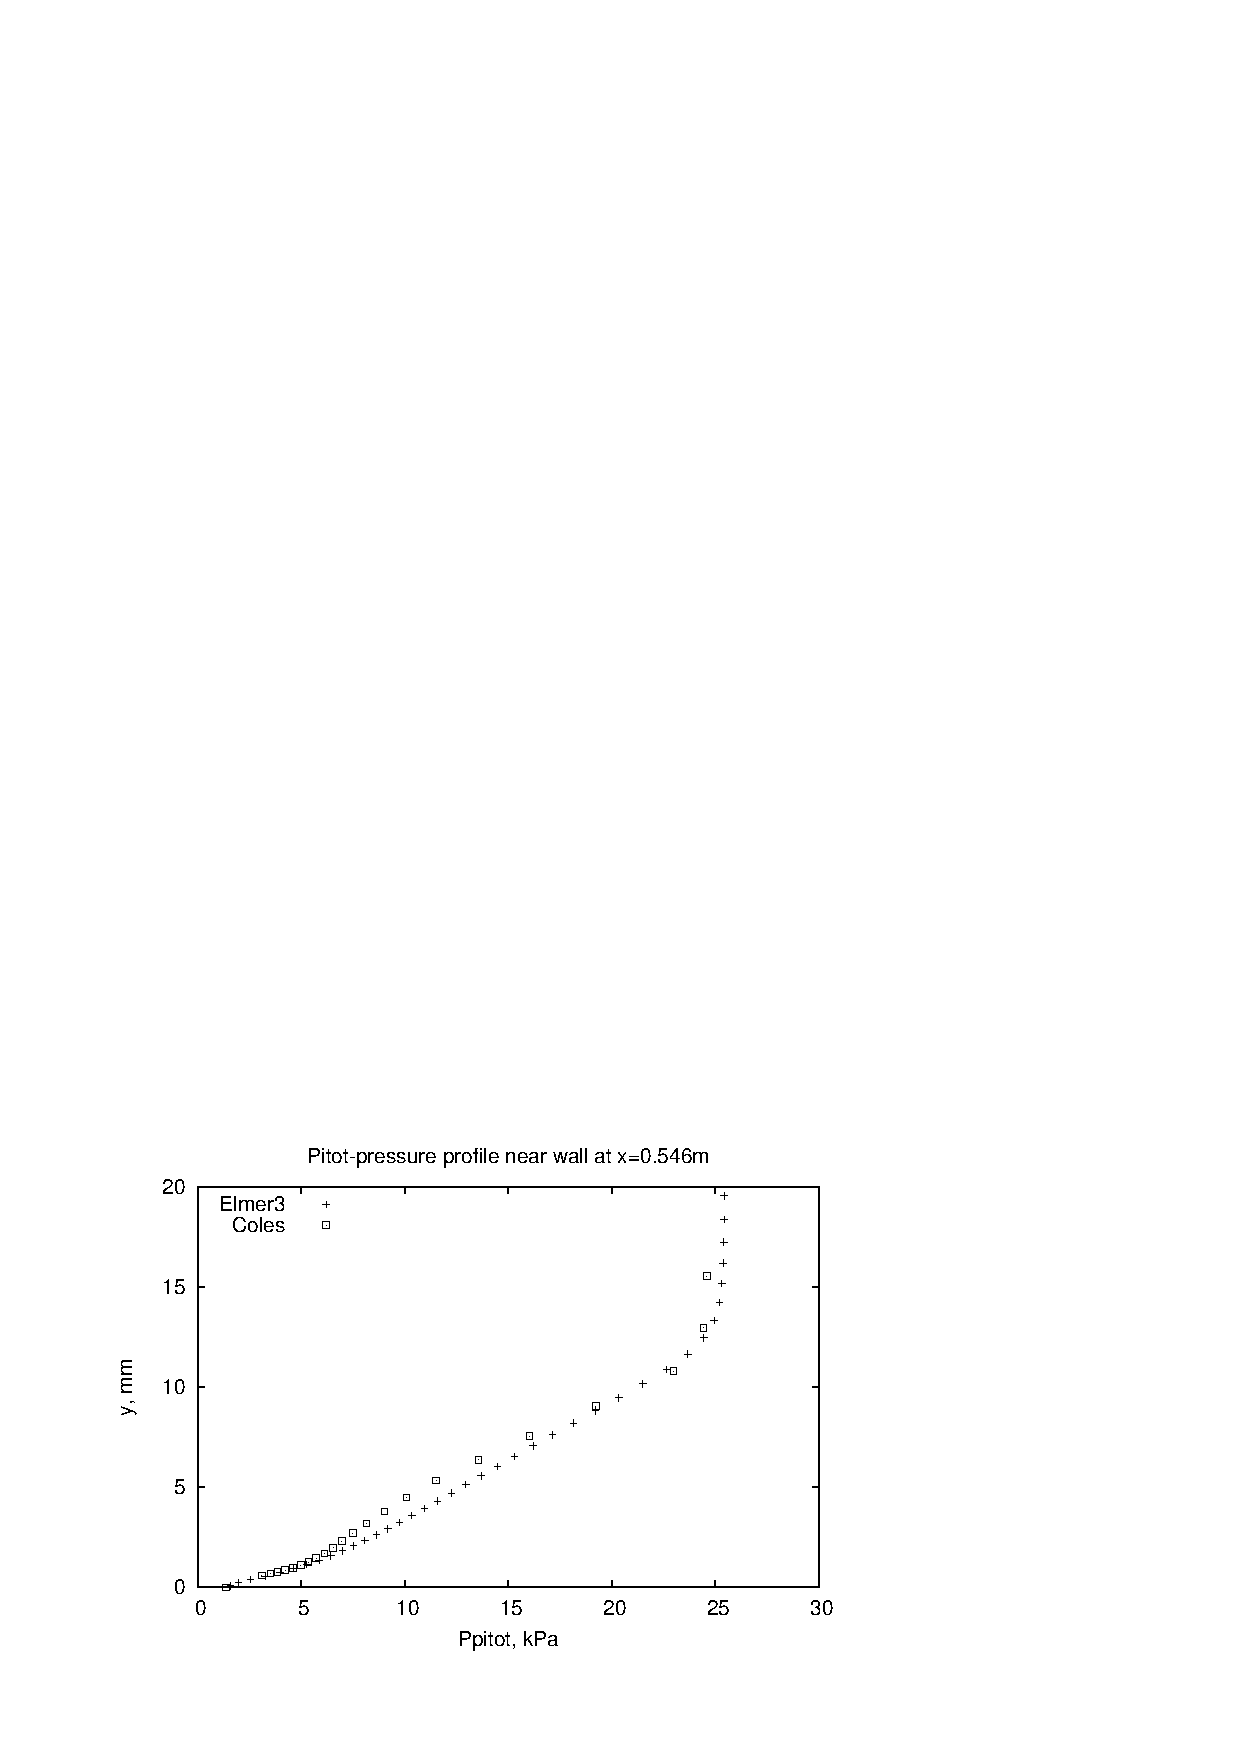
\includegraphics[width=7cm]{./chap2-flat-plate/figs/coles-x05-pitot.png}
% }
% \subfigure[Caption for second subfigure]{
%   \label{SecondSubFigure}
%   \fbox{Contents of second subfigure}
% 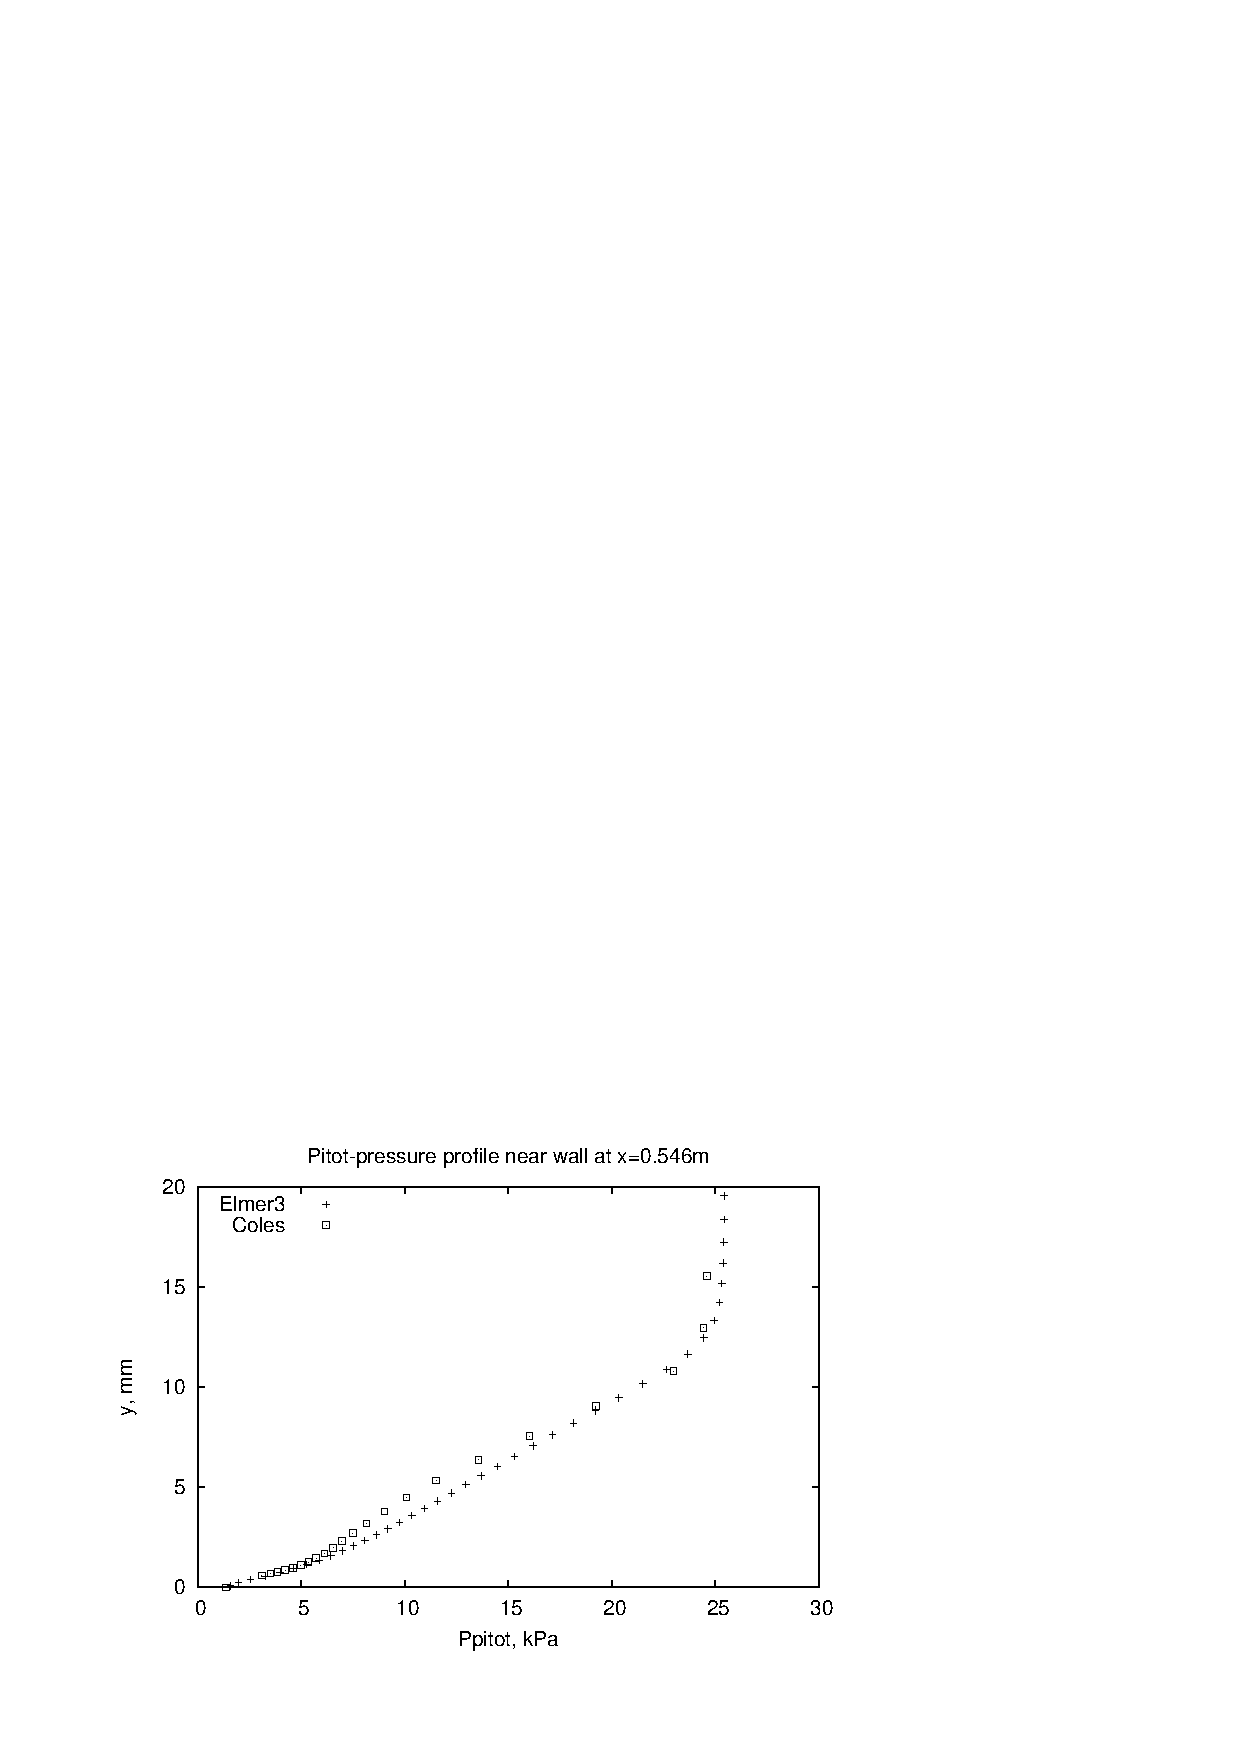
\includegraphics[width=7cm]{./chap2-flat-plate/figs/coles-x05-pitot.png}
% }
% \caption{Caption for the overall figure}
% \label{grid-convergence-fig}
%\end{figure}
%------------------------------------------------------------------
\subsection{Sensitivity to freestream turbulence properties}
\label{flat-plate-sensitivity}
%
The $k$-$\omega$ model has been known to be sensitive to the freestream 
values of turbulence properties. To assess this sensitivity, values of 
freestream turbulence intensity and turbulent-to-laminar viscosity ratio 
have been varied within the recommended range previously discussed in 
Section~\ref{section-intro-recommended-guidelines}. Table~\ref{sensitivity-study-matrix} 
shows a matrix of test cases set up to examine this sensitivity. 
Figures~\ref{flat-plate-BL-profile-546mm} and \ref{flat-plate-cf} show the computed boundary layer profiles
at $x$ = 0.546 m and the values of skin friction coefficient along the wall respectively for the nine test cases.
The boundary layer profiles and skin friction coefficient values show that the $k$-$\omega$ model 
is indeed sensitive to the values of freestream turbulence properties, with the largest variations
in the pitot pressure and density profiles. The skin friction coefficient plot also reveals that
the boundary layer may be transitioning at different locations for different freestream turbulence properties.
This indicates that the variation in boundary layer profiles for the nine cases 
in Figures ~\ref{flat-plate-BL-profile-546mm} 
and \ref{flat-plate-cf} could also be partially brought about by the difference
in the boundary layer transitioning location. The effect of the $k$-$\omega$ model's sensitivity to freestream 
turbulence properties will be further discussed during the comparison of the numerical and experimental results
in Section~\ref{flat-plate-results-and-discussions}.
\begin{table}[h]
  \caption{Test matrix for the study of turbulence model sensitivities}
  \label{sensitivity-study-matrix}
  \begin{center}
    \begin{tabular}{ccccl}
      \hline\hline
      & \multicolumn{3}{c}{Turbulence Intensity} \\
      \hline
      $\mu_t/\mu$ & 1.0\%  & 5.0\%  & 10.0\% \\
      \hline
      1.0     &  Case 1    &  Case 4    &  Case 7   \\
      10.0    &  Case 2    &  Case 5    &  Case 8   \\
      100.0   &  Case 3    &  Case 6    &  Case 9   \\
      \hline \hline
    \end{tabular}
  \end{center}
\end{table}
%
\begin{figure}[h]
 \centering
 \subfigure[Pitot pressure]{
   \label{flat-plate-pitot}
%   \fbox{Contents of first subfigure}
   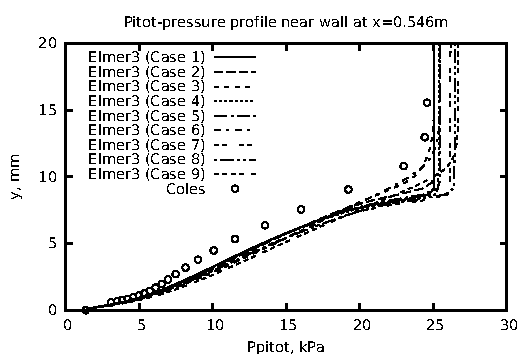
\includegraphics[width=7cm]{./chap2-flat-plate/figs/coles-x-546-pitot.pdf}
 }
 \subfigure[Density]{
   \label{flat-plate-density}
%   \fbox{Contents of second subfigure}
 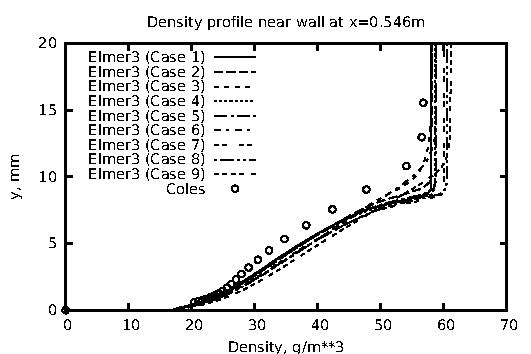
\includegraphics[width=7cm]{./chap2-flat-plate/figs/coles-x-546-density.pdf}
 }
 \subfigure[Temperature]{
   \label{flat-plate-temperature}
%   \fbox{Contents of first subfigure}
   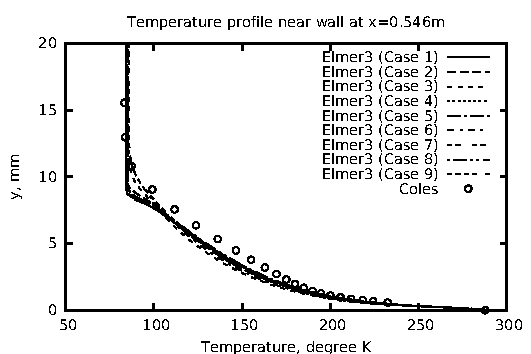
\includegraphics[width=7cm]{./chap2-flat-plate/figs/coles-x-546-temperature.pdf}
 }
 \subfigure[$u$-velocity]{
   \label{flat-plate-u-velocity}
%   \fbox{Contents of second subfigure}
 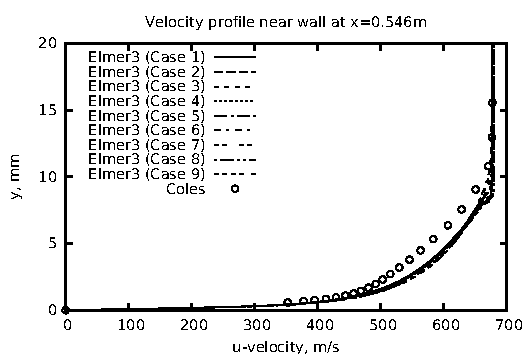
\includegraphics[width=7cm]{./chap2-flat-plate/figs/coles-x-546-u.pdf}
 }
 \caption{Near-wall boundary layer profiles at $x$ = 0.546 m}
 \label{flat-plate-BL-profile-546mm}
\end{figure}
%
\begin{figure}[h]
 \begin{center}
  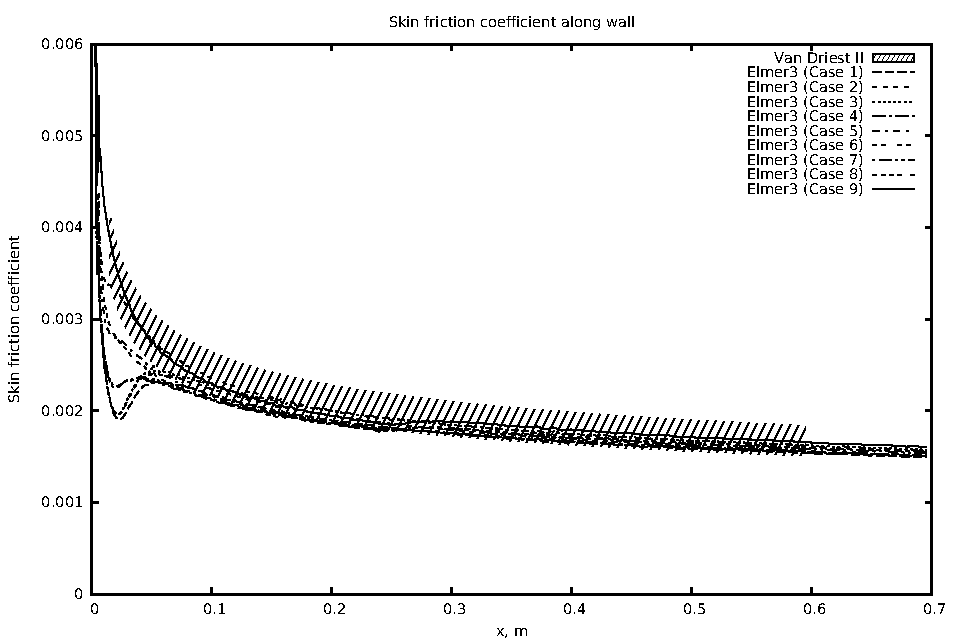
\includegraphics[width=12.5cm]{./chap2-flat-plate/figs/coles-x-cf.pdf}
 \end{center}
 \caption{Skin friction coefficient along flat plate}
 \label{flat-plate-cf}
\end{figure}

%------------------------------------------------------------------
\subsection{Results \& discussions}
\label{flat-plate-results-and-discussions}
%
Figures~\ref{flat-plate-BL-profile-546mm} and \ref{flat-plate-BL-profile-646mm} 
show the comparison between the experimental and numerical boundary layer 
profiles at $x$ = 0.546 m and $x$ = 0.646 m respectively. It can be seen that 
the profiles at $x$ = 0.646 m match the experimental data better than those at 
$x$ = 0.546 m, even though the experimental profiles were sampled at $x$ = 0.546 m.
There is a certain level of uncertainty regarding the way the boundary layer transitions with
the boundary layer trip used in the experiments. In addition, this method of tripping the
boundary layer may not be accurately modelled by the turbulence model. The use of 
non-dimensionalised flow variables should somewhat alleviate this issue. 
Figure~\ref{flat-plate-dimensionless-velocity} shows the non-dimensionalised 
velocity against the non-dimensionalised distance from the wall. It can be
seen that the dimensionless velocity profiles at both locations match each other, and also the
incompressible logarithmic law-of-the-wall velocity profile.
%
\begin{figure}[h]
 \centering
 \subfigure[Pitot pressure]{
   \label{flat-plate-pitot}
%   \fbox{Contents of first subfigure}
   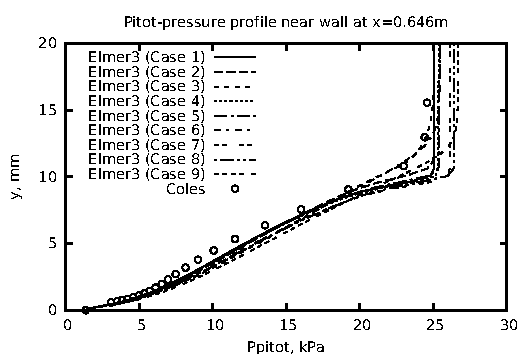
\includegraphics[width=7cm]{./chap2-flat-plate/figs/coles-x-646-pitot.pdf}
 }
 \subfigure[Density]{
   \label{flat-plate-density}
%   \fbox{Contents of second subfigure}
 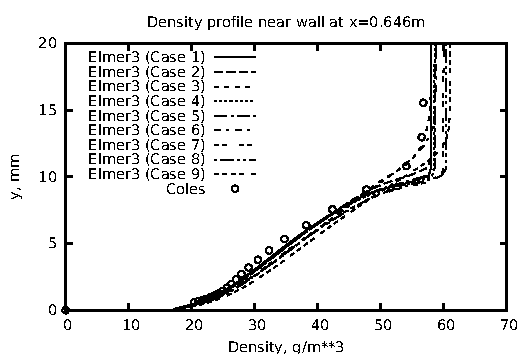
\includegraphics[width=7cm]{./chap2-flat-plate/figs/coles-x-646-density.pdf}
 }
 \subfigure[Temperature]{
   \label{flat-plate-temperature}
%   \fbox{Contents of first subfigure}
   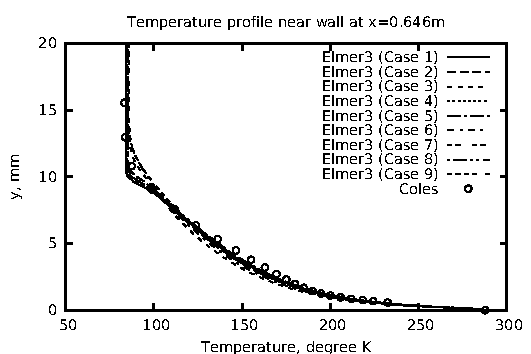
\includegraphics[width=7cm]{./chap2-flat-plate/figs/coles-x-646-temperature.pdf}
 }
 \subfigure[$u$-velocity]{
   \label{flat-plate-u-velocity}
%   \fbox{Contents of second subfigure}
 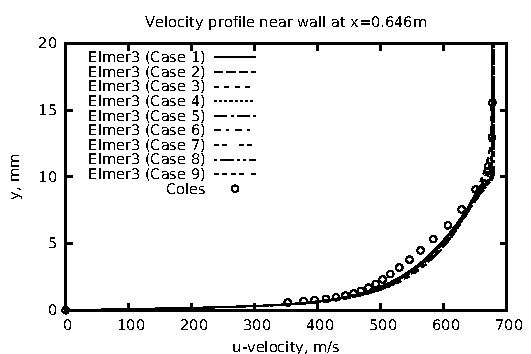
\includegraphics[width=7cm]{./chap2-flat-plate/figs/coles-x-646-u.pdf}
 }
 \caption{Near-wall boundary layer profiles at $x$ = 0.646 m}
 \label{flat-plate-BL-profile-646mm}
\end{figure}
%
\begin{figure}[h]
 \begin{center}
  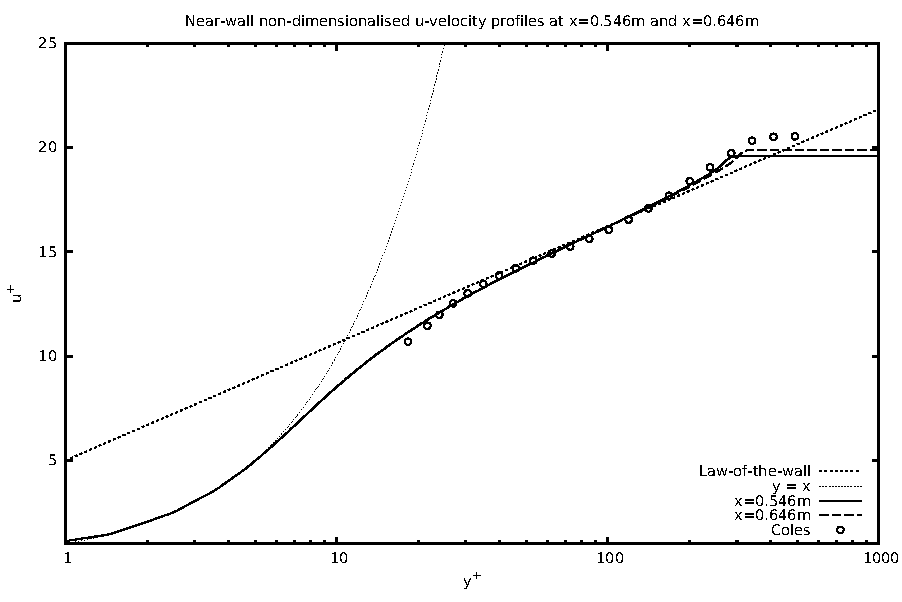
\includegraphics[width=12.5cm]{./chap2-flat-plate/figs/coles-x-dimensionless.pdf}
 \end{center}
 \caption{Non-dimensionalised velocity profiles}
 \label{flat-plate-dimensionless-velocity}
\end{figure}
%
Figure~\ref{flat-plate-cf} shows a comparison between the skin friction coefficient 
computed using van Driest's turbulent skin friction theory and computed using Eilmer3. 
Using an uncertainty band of $\pm$10\% for the theoretical plot, it can be seen that 
the numerical results are within the uncertainty band of van Driest's turbulent skin 
friction theory. This shows that the $k$-$\omega$ model in Eilmer3 can be used to 
predict turbulent skin friction coefficient on a flat plate, despite the model's 
sensitivity to freestream turbulence properties.
%------------------------------------------------------------------
